\chapter{GPU 内存模型之 Proxy}

\begin{center}\small 作者：reed（知乎 @reed-84-49，专栏「CUDA高性能编程」）\quad 原文：\url{https://zhuanlan.zhihu.com/p/2080760925481592736}\end{center}

C++ 内存模型用 happens-before 表达跨线程的数据交接：release 与 acquire 配对后，release 之前的普通写入可以由 acquire 之后的读取安全观察。编译器与硬件负责把这一语言级关系映射到目标平台；访问方法本身不会作为独立维度暴露给程序。

GPU 为提高数据搬运效率引入了多套硬件通路。除通用 LD/ST 单元外，TMA 按描述符独立搬运 global 与 SMEM 之间的数据，Tensor Core 也有直接访问 SMEM 的操作数通路。这些通路各有队列与执行单元，PTX 不假定它们天然共享同一个访存顺序，而是把访问方法的差异抽象为 proxy。

由此，release/acquire 不能单独跨越不同 proxy 建立顺序；跨 proxy 数据边必须先由 proxy fence 或指令规定的隐式机制建立 causality。proxy fence 的方向由 from $\rightarrow$ to 固定，与 \lstinline|.release| / \lstinline|.acquire| 无关。若两个操作还分属不同线程，再由 release/acquire 与 scope 建立线程间同步。线程关系与访问方法因此是正交的——同一线程先后发出的两个操作，只要分属不同通路，程序序也不能替代 cross-proxy ordering。

mbarrier 进一步把“事务完成”与“内存可见性”拆成两件相互独立的事：计数决定完成，同步语义决定可见性。异步流水线的同步因此可以分解为依次确认的四步：Q1 用计数机制确认异步事务完成，Q2 确定消费方所经的 proxy 以及它必须看到的内容，Q3 按正向交接的普通内存端点所跨的线程范围选择 scope，Q4 判断缓冲区的反向复用是否跨 proxy。其中 Q2 同时覆盖可见性与 cross-proxy ordering，tcgen05 等异步指令族在这一步附加各自的 execution ordering；Q4 在同 proxy 时保留相应的完成与 execution ordering，跨 proxy 时再补反向 fence。

行文上，先从 C++ 内存模型出发，引入 proxy 的硬件基础与 morally strong 三条件，说明线程与访问方法两个维度为什么正交；再梳理 fence、barrier 与 mbarrier 的分工；随后逐一走过四种典型数据边，最后给出同步判定的四步流程与总结。

\section{C++ 内存模型}

\section{契约、实现与数据竞争}

内存模型规定一个线程的写在什么条件下能够被另一个线程观察。它描述可见性与顺序，不规定操作发生的物理时刻；“程序顺序 = 执行顺序 = 可见顺序”在现代系统中并不成立。内存模型是契约而非机制，编译器、流水线与缓存一致性协议共同实现这份契约。

三层的职责划分如图 1 所示：编译器负责把语言级的顺序要求翻译成指令与屏障，并放弃契约所禁止的优化；流水线与 store buffer 负责跨地址的访存顺序以及 fence 的语义；缓存一致性协议则按每个地址维持单写多读与数据值不变式。

\begin{figure}[htbp]\centering
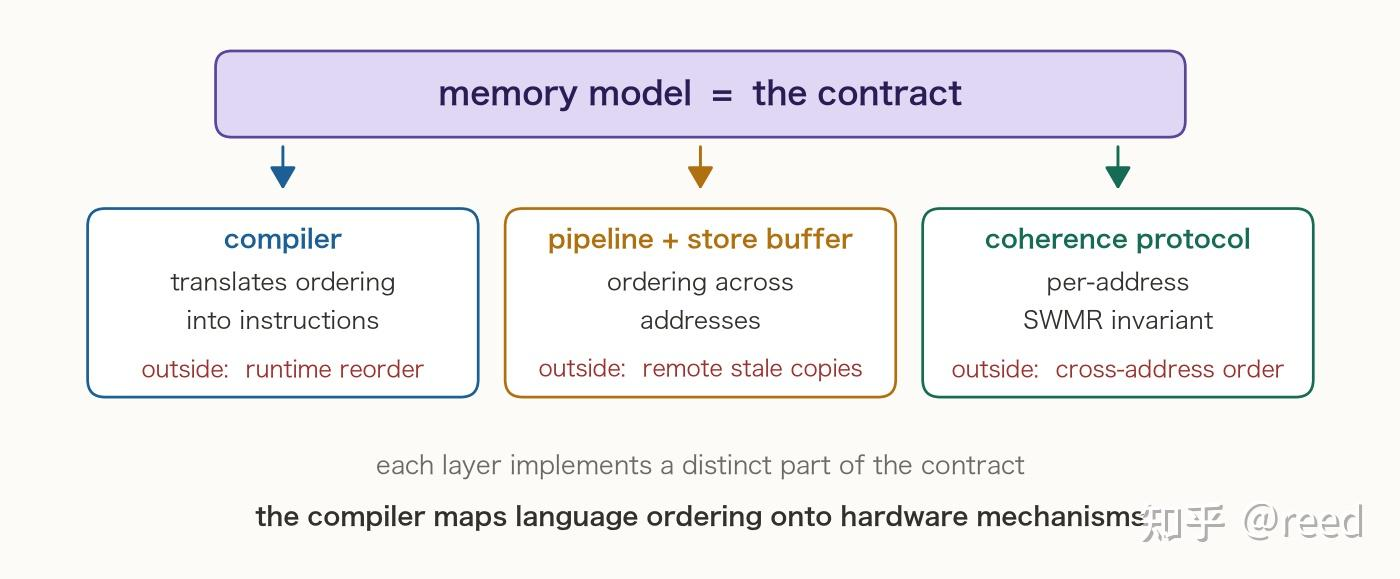
\includegraphics[width=0.9\textwidth]{figures/reed-mem-01-proxy/fig-01.jpg}
\caption{Figure 1. The contract and its three implemention}
\end{figure}

图中三根箭头指向的三张卡片，正是契约的三个实现者，卡片下方的红字标出各自管不到的部分——每一层都只兑现契约的一部分，任何一层都无法独力提供跨线程可见性。一致性协议维护单一地址的副本状态，但不规定不同地址写入的相对可见顺序，这一层顺序需要由 fence 建立；流水线可以约束本地发射顺序，却不能替代缓存一致性协议的传播职责。语言模型与硬件内存模型之间还隔着编译器翻译：目标指令序列提供的保证不得弱于语言契约，硬件模型越弱，编译器需要插入的真实同步指令越多。

对本文讨论的普通对象读写，C++ 数据竞争的判据是：两个潜在并发的操作访问同一内存位置，且至少一个为写，称为冲突；若至少一个操作不是原子操作，二者又没有 happens-before 关系，则构成数据竞争，程序行为未定义。

\begin{quote}
潜在并发 + 冲突 + 至少一方非原子 + 无 happens-before = 数据竞争。
\end{quote}

\section{happens-before}

忽略本文不讨论的 \lstinline|memory_order_consume| 后，happens-before 可由两部分合成并取传递闭包：

\begin{lstlisting}
happens-before = (sequenced-before and synchronizes-with)
\end{lstlisting}

其中 sequenced-before 是单线程内的程序顺序，它指的是语义上的先后，而非指令发射的先后；synchronizes-with 则是跨线程的那条边，由 release 与 acquire 配对、mutex、thread join 等操作建立。

二者的分工由此清楚：单线程内部由 sequenced-before 确定抽象机中的先后关系；一旦跨越线程，程序顺序不再延伸过去，普通共享数据的交接必须由 synchronizes-with 建立 happens-before。

happens-before 约束后续操作可以观察哪些副作用；对普通共享数据而言，它是跨线程无竞争交接的前提，原子对象的取值还需满足各自的 modification order。由于该关系可传递，一条 release/acquire 边可以覆盖 release 之前的多次写入，无需为每个数据对象单独建立同步。

\begin{figure}[htbp]\centering
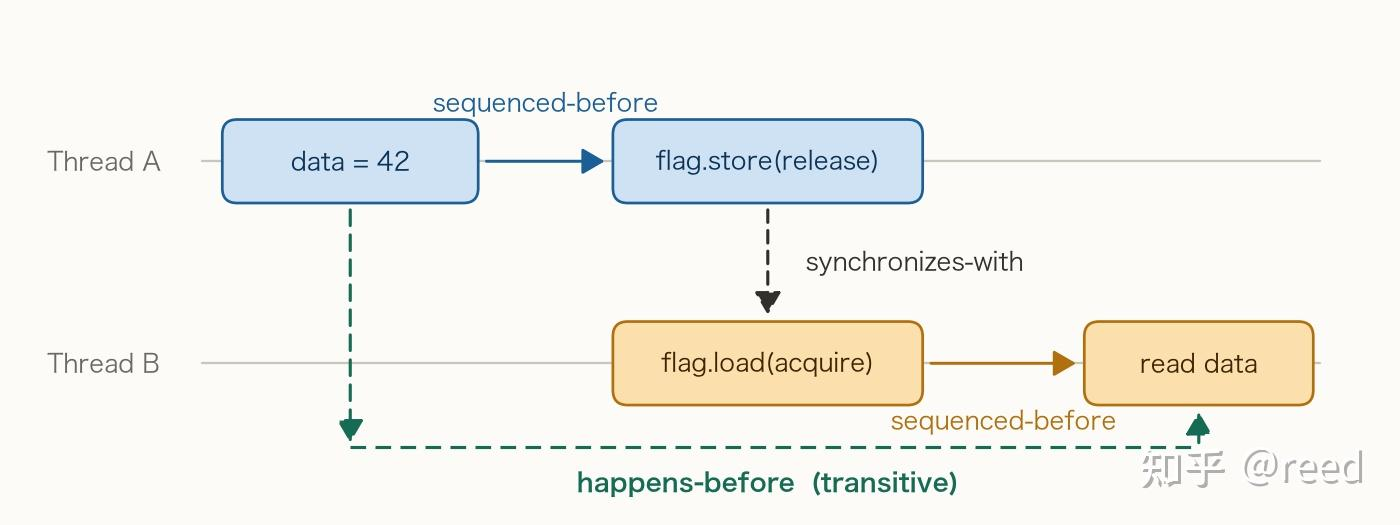
\includegraphics[width=0.9\textwidth]{figures/reed-mem-01-proxy/fig-02.jpg}
\caption{Figure 2. Composing happens-before from sequenced-before and synchronizes-with.}
\end{figure}

图中两条实线是各自线程内的 sequenced-before，中间那条虚线是由 release/acquire 建立的 synchronizes-with；三段首尾相接，才把线程 A 的 data = 42 排到线程 B 的读取之前。缺了中间那条跨线程边，两侧的程序序无法拼成一条 happens-before。

\section{acquire / release / relaxed}

C++ 有六种 \lstinline|memory_order|，常用四种，核心区别在约束方向：

relaxed 只保证原子对象自身的原子性与 modification order，不对周围访问增加同步约束；release 与 acquire 典型地分别用于 store 和 load，前者约束其前序读写，后者约束其后续读写，原子 RMW 与 fence 也可以携带相应语义；所有 \lstinline|seq_cst| 操作在此之上构成单一总序，通常不需要使用这一更强约束。

\begin{figure}[htbp]\centering
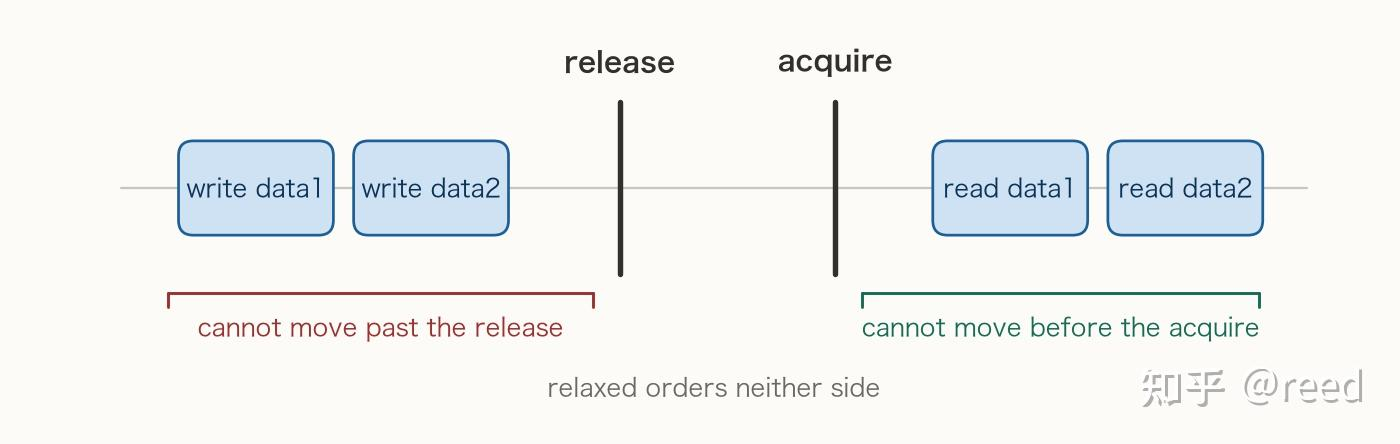
\includegraphics[width=0.9\textwidth]{figures/reed-mem-01-proxy/fig-03.jpg}
\caption{Figure 3. A release orders what precedes it; an acquire orders what follows it.}
\end{figure}

\begin{lstlisting}
// 线程 A（生产者）
data = 42;
flag.store(true, std::memory_order_release);

// 线程 B（消费者）
while (!flag.load(std::memory_order_acquire)) {}
assert(data == 42);                              // 一定成立
\end{lstlisting}

把 release 换成 relaxed 后，data 的非原子读写之间没有 happens-before，程序产生数据竞争并进入未定义行为；问题并非仅仅是某次 assert 失败。

方向性为：release 约束其前序访问，acquire 约束其后续访问。

\section{fence}

fence 约束同一线程中位于其前后的访存顺序，不要求其它线程到达某个执行点。单独的 fence 不构成跨线程同步边；跨线程传递数据仍需一次可被对端观察的通信操作，例如作用于同一原子对象的写入与读取。fence 负责约束通信操作两侧的顺序，通信操作负责把可见性关系连接到另一线程。

在实现层面，编译器需要禁止跨越 fence 的相关重排，硬件需要等待前序访存满足目标内存模型要求。具体指令和开销由目标体系结构决定；这层抽象足以对应 PTX 中 thread fence 与 release/acquire pattern 的作用。到了 GPU，还要处理一个 C++ 模型中不存在的维度：访问方法本身也成为内存模型必须显式定序的对象。

\section{Proxy 的硬件基础}

\section{Coherence 与 consistency}

coherence 与 consistency 描述不同层次的问题（Nagarajan、Sorin、Hill、Wood，A Primer on Memory Consistency and Cache Coherence）。coherence 按单一内存位置定义，维护该地址副本的单写多读与数据值不变式；consistency 面向多个地址，规定不同线程可以观察到的跨地址顺序。coherence 约束单一地址的写入传播，consistency 约束多个地址之间的可见顺序。

对本文而言，关键变化是 PTX 不假定不同访存方法共享同一个一致视图。DMA 类单元与线程 LD/ST 可以访问同一地址，却经由不同队列和端口；跨方法顺序必须由内存模型显式建立，proxy 正是对此的抽象。

\section{Proxy 与访存方法}

C++ 内存模型不把访问方法作为独立维度暴露给程序。GPU 则在单个 SM 上提供多套物理独立的访存通路：通用 LD/ST 单元（线程执行 \lstinline|ld/st/atom|）、TMA 引擎（执行 \lstinline|cp.async.bulk*| 的 DMA 式搬运单元）、Tensor Core 操作数通路（\lstinline|tcgen05.mma| 直接从 SMEM 取 A/B）、TMEM 通路（\lstinline|tcgen05.ld/st|）。

这些通路分别优化不同的数据路径：TMA 将地址计算与边界处理交给硬件并允许搬运与计算重叠，Tensor Core 直接从 SMEM 获取操作数，TMEM 为累加器提供独立于寄存器堆的存储。各通路拥有独立的队列与缓冲，其中几条还落在同一块物理 SRAM 上、抵达路径彼此独立；PTX 不假定它们共享统一的访存视图，而是将访问方法的差异抽象为 proxy。

PTX 列出的非 generic 访问方法包括 texture / surface、alias、async、tensormap 与 fabric。本文主要涉及 generic 与 async：普通 ld、st、atom、red 和 mbarrier 指令属于 generic proxy，\lstinline|cp.async.bulk*| 以及 \lstinline|tcgen05.mma| / \lstinline|tcgen05.cp| 对 SMEM 的访问属于 async proxy。用不同虚拟地址访问同一位置虽然仍采用 generic 方法，也按跨 proxy（\lstinline|.alias| proxy）处理。

\section{四个基本构件}

异步搬运的完成经由单元到单元的消息路径回报。 线程提交 TMA 时只递交描述符（tensormap + 坐标）就返回，搬运由引擎独立完成，完成后按 \lstinline|mbarrier::complete_tx::bytes| 对屏障做一次事务计数（tx-count）归减。这条回报路径不属于线程指令流，线程因此无法凭自身的程序序判断搬运何时结束。

scope 定义同步直接覆盖的线程集合。 \lstinline|.cta| 覆盖与当前线程同属一个 CTA 的线程，\lstinline|.cluster|、\lstinline|.gpu| 与 \lstinline|.sys| 再依次扩大到同一 cluster、整个 device 与系统范围。同一 SM 可以同时驻留多个 CTA，因此 \lstinline|.cta| 不是 SM scope。PTX 只承诺相应线程集合中的可见性与顺序，具体需要刷新、失效或穿越哪些缓存层级由实现决定。这一点对普通写同样适用：一次写可以先在较小的 scope 内可见，再传播到更大范围，程序员需要确定的是同步必须覆盖哪些线程。

mbarrier 是 SMEM 中的 8 字节状态对象。 \lstinline|.layout::v0| 与 \lstinline|.layout::v1| 都维护 pending arrival count、tx-count 与 primary / conditional phase；arrive-on 和 \lstinline|complete_tx| 分别递减前两个计数，满足当前 phase 的完成条件后对象自动进入下一 phase。v1 额外维护 payload report，并允许异步操作阻止 conditional phase 推进；本文只使用默认的 v0，其 primary 与 conditional phase 同步前进。mbarrier 位于 SMEM，因此 cluster 内其它 CTA 可以通过 DSMEM（distributed shared memory，cluster 内 CTA 之间可互相寻址的 SMEM）地址执行 arrive；\lstinline|test_wait| / \lstinline|try_wait| 仅支持本 CTA 的 mbarrier 对象，因为等待操作还涉及本 SM 上线程的挂起与恢复。

fence 建立内存模型要求的顺序。 线程 fence 约束同一线程在指定 scope 内的访存顺序；proxy fence 则在两种访存方法之间建立 cross-proxy causality order。PTX 只定义这种顺序及其可见性效果，具体硬件可能表现为等待队列排空、阻止后续发射或同步内部状态。

与 C++ 抽象机相比，PTX 额外暴露了两个选择：同步直接覆盖哪些线程，以及访问是否跨 proxy。前者由 scope 表达，后者由 proxy fence 处理；二者分别对应线程维度和访存方法维度。下一节说明，这两个维度为什么是正交的。

\section{Proxy 与线程的正交}

PTX 用 causality order 描述跨操作的因果先后，它在功能上承担类似 C++ happens-before 的角色，但正式定义还包含 PTX 特有的 proxy-preserved base causality 与 observation order，二者并不等同。release/acquire pattern 是跨线程建立 synchronizes-with 的一种形式，morally strong 是这类 synchronizes-with 成立时的端点条件，也是多数 PTX 内存模型公理使用的关系条件；其中 strong 描述操作的内存语义与 scope，不表示执行时延或硬件强度。

PTX 规定，两个操作要构成 morally strong 必须同时满足三个条件：二者要么由同一线程按程序序执行，要么各自都是 strong 操作且 scope 互含对方线程；二者必须经由同一个 proxy；若都是内存操作，则必须完全重叠（PTX ISA，Memory Consistency Model: Morally Strong Operations）。

这三个条件的地位并不相同。第一个条件有两种满足方式，同一线程按程序序执行即可满足；第二个与第三个条件则在所有情形下都必须满足。这一差别决定了 proxy 与线程是两个正交的维度：即便两个操作出自同一个线程、在程序中一前一后，只要它们经由不同的 proxy，morally strong 依然不成立。程序序仍然存在，但不足以建立跨 proxy 的 causality 与内存可见性；这一额外维度在 C++ 模型中没有对应物，因为那里不把访问方法暴露给程序。

synchronizes-with 要求 release pattern 的首操作与 acquire pattern 的末操作 morally strong，因此可以得到：

\begin{quote}
release/acquire 单独不能为跨 proxy 的两个操作建立 causality order。
\end{quote}

C++ 与 PTX 对 data race 的正式定义并不相同：C++ 关注潜在并发的非原子冲突是否缺少 happens-before，PTX 则要求冲突访问既没有 causality order、又不 morally strong。proxy 出现在 PTX 的第二个条件中；只有在 cross-proxy causality 也未建立时，冲突访问才形成 PTX data race。

一个 \lstinline|mbarrier.try_wait| 上的 \lstinline|.acquire| 本身不是 proxy fence，不能单独建立 generic 与 async 之间的 ordering。对 TMA 写入而言，completion 已经提供 async$\rightarrow$generic 的隐式 proxy ordering（详见下文“TMA 完成语义”），成功的 acquire wait 再把后续 generic 读取排在完成之后，因此不需要额外执行显式 \lstinline|fence.proxy.async|。

proxy fence 建立的是 cross-proxy causality，而 release/acquire 建立的是跨线程 synchronizes-with。若操作出自同一线程，只需补足缺失的 cross-proxy ordering；若操作还分属不同线程，则两类关系都要成立。async 指令在请求完成前即把控制权返回给执行线程，generic 与 async 通路因此可以并行推进；cross-proxy ordering 约束的正是这两条通路之间的可见顺序。

\begin{figure}[htbp]\centering
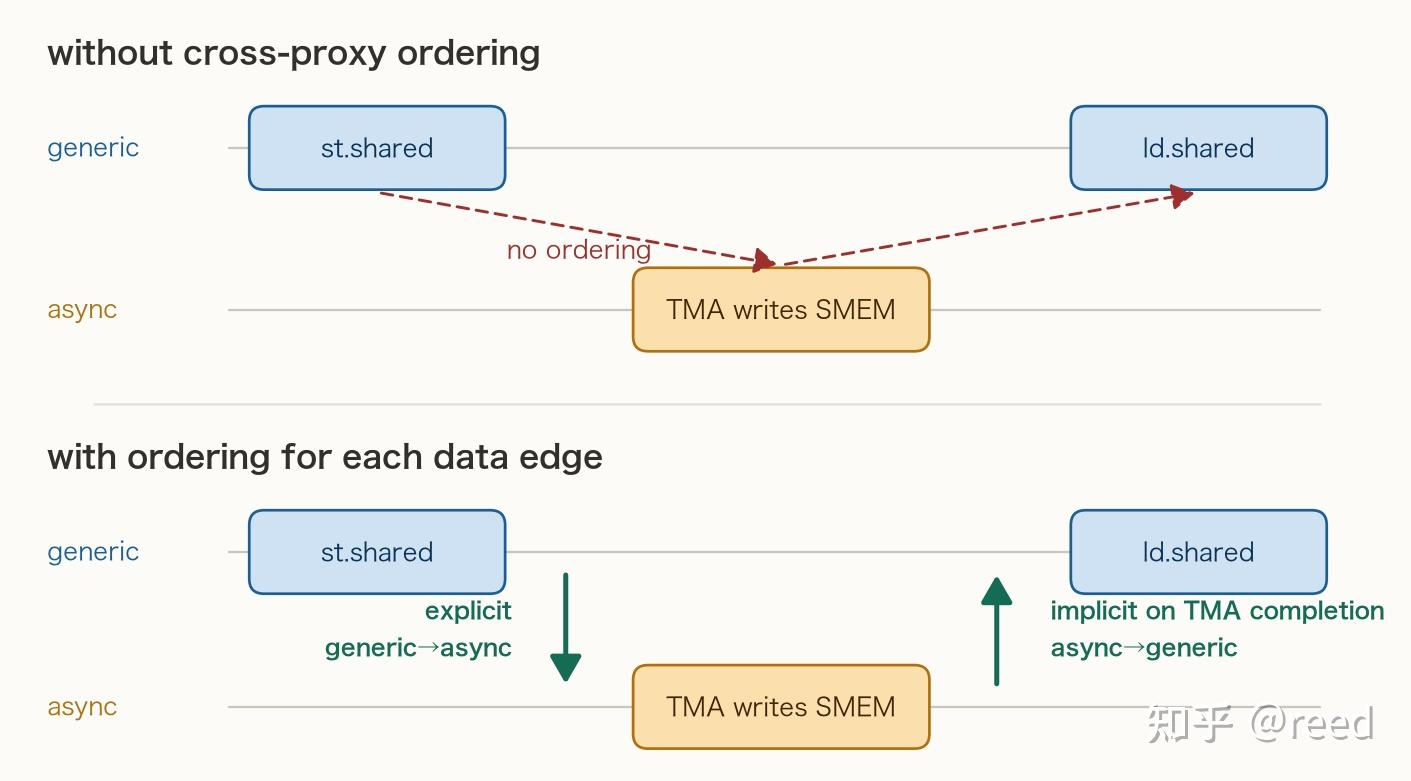
\includegraphics[width=0.9\textwidth]{figures/reed-mem-01-proxy/fig-04.jpg}
\caption{Figure 4. Cross-proxy ordering must be established in the direction of each data edge.}
\end{figure}

上图是无 fence 的情形：同一块地址被 generic 线与 async 线交替访问，两次访问之间不存在任何排序关系。下图为每条数据边各建立一个方向的 cross-proxy ordering 后，两个方向分别被定序；其中 async$\rightarrow$generic 由 TMA 完成隐式提供，generic$\rightarrow$async 才需要显式 fence。

\section{GPU 上的同步原语与可见性}

\section{三类原语的分工}

fence、barrier 与 mbarrier 分别解决访存定序、线程会合和事件或事务完成三个问题，职责如图 5 所示。

\begin{figure}[htbp]\centering
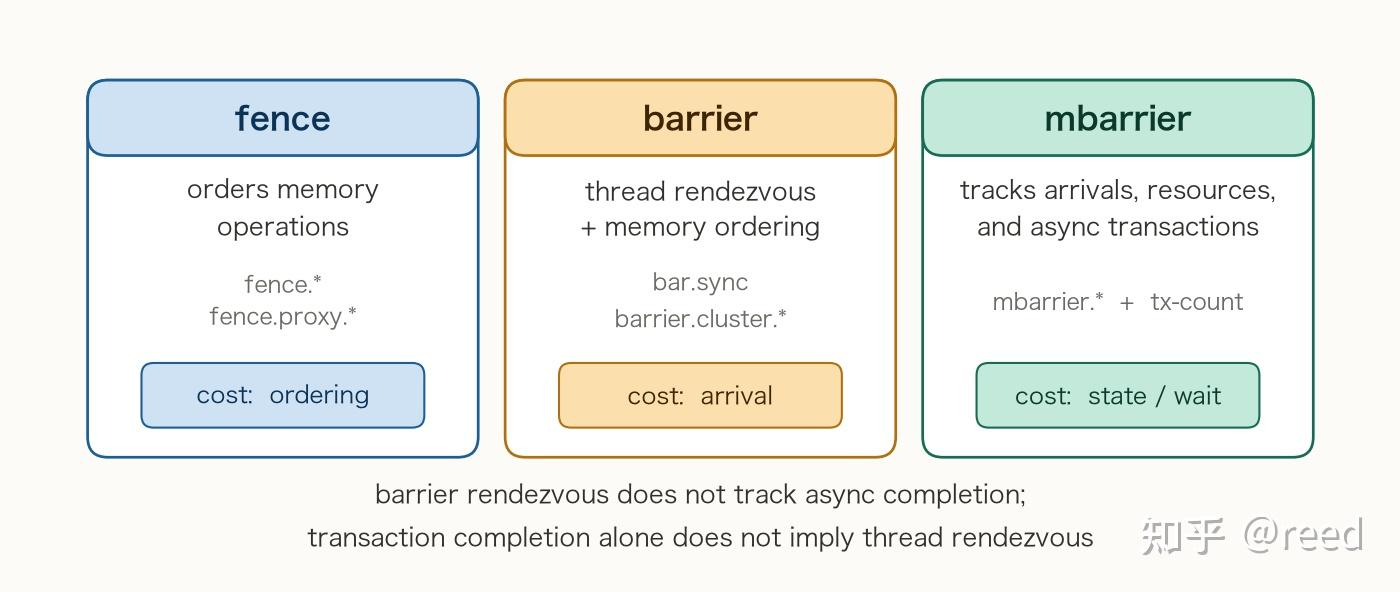
\includegraphics[width=0.9\textwidth]{figures/reed-mem-01-proxy/fig-05.jpg}
\caption{Figure 5. Three primitives for three distinct problems}
\end{figure}

CUDA barrier 同时提供执行同步与内存可见性保证。 \lstinline|__syncthreads()| 首先等待线程块内所有未退出线程到达同一同步点；barrier 完成后，参与线程在 barrier 之前发起的普通内存访问（ld / st / atom / red，不含 TMA、cp.async、tcgen05 等异步事务）已经完成，并对这些线程从 barrier 返回后的访问可见。异步事务的完成必须由 mbarrier 或相应的 \lstinline|*.wait_group| 另行确认。因此，barrier 的作用包含两个不可分割的部分：线程在执行进度上会合，以及会合前的普通内存效应对参与线程可见。PTX 的 \lstinline|bar.sync| 提供相应语义。

mbarrier 与前两者的区别在于把 arrival 与 wait 拆开：以 expected arrival count 定义每个 phase 需要满足的 arrival 数量，并可同时跟踪 tx-count；实际参与线程由控制流决定，同一线程也可以贡献多个 arrival。当参与线程分别 arrive 并等待同一 phase 时，mbarrier 可以实现 split-phase 线程会合。仅等待异步事务完成或资源状态的 mbarrier 用法不自动代表某个线程集合已经会合，而普通 barrier 也不提供 TMA 的事务完成跟踪。

\section{Scope 作为同步条件}

release 的 scope 必须包含 acquire 线程，acquire 的 scope 也必须包含 release 线程；跨 CTA 的普通数据交接因此要求两侧都使用 \lstinline|.cluster|，单边升级不能建立所需关系。

scope 与地址空间相互独立。\lstinline|.shared::cluster| 表示 mbarrier 对象或数据位于可由 cluster 访问的 SMEM 地址空间，\lstinline|.scope::cluster| 表示同步效果覆盖 cluster 内线程；访问远端地址不自动把同步 scope 升为 cluster，访问本地地址也不代表 CTA scope 必然充分。判断依据始终是 release 与 acquire 的执行端点及需要传递的内存效应。

\section{Fence 家族}

PTX 里 fence 有四类：

\begin{lstlisting}
// 1) 线程 fence：约束本线程访存之间的顺序
fence{.sem}.scope;
fence.acquire.sync_restrict::shared::cluster.cluster; // 只针对 shared::cluster 空间
fence.release.sync_restrict::shared::cta.cluster;

// 2) 操作 fence：只针对某一类操作（.op_restrict = { .mbarrier_init }）
fence.mbarrier_init.release.cluster;

// 3) proxy fence（双向）：为两条 proxy 线互相定序，不带 scope
fence.proxy.proxykind; // 例：fence.proxy.async.shared::cta

// 4) proxy fence（单向）：只约束一个方向，带 scope
fence.proxy.to_proxykind::from_proxykind.release.scope;
fence.proxy.to_proxykind::from_proxykind.acquire.scope [addr], size;
fence.proxy.async::generic.release.sync_restrict::shared::cta.cluster;
fence.proxy.async::generic.acquire.sync_restrict::shared::cluster.cluster;
\end{lstlisting}

\lstinline|fence.proxy.to::from| 的方向始终由 from $\rightarrow$ to 决定。因而 \lstinline|fence.proxy.async::generic.release| 与 \lstinline|fence.proxy.async::generic.acquire| 都建立 generic$\rightarrow$async 的单向 proxy ordering；\lstinline|.release| 与 \lstinline|.acquire| 决定的是这两条 fence 如何组成跨线程的 release/acquire sequence，并不会把 proxy 方向反转。无需区分方向时可以使用双向 \lstinline|fence.proxy.async|。

\lstinline|.sync_restrict| 是可选限定符，一旦出现就与 \lstinline|.sem| 强绑定：\lstinline|.sync_restrict::shared::cta| 只能配 \lstinline|.release|，\lstinline|.sync_restrict::shared::cluster| 只能配 \lstinline|.acquire|，且此时 \lstinline|.scope| 必须为 \lstinline|.cluster|，fence 的作用范围被限制在对应地址空间的对象上；省略 \lstinline|.sync_restrict| 时 fence 作用于所有状态空间。因此像 acquire + \lstinline|sync_restrict::shared::cta| 这样的组合并不合法。规范没有解释这条不对称从何而来，但官方示例给出了用法上的分工：release 侧要发布的是本 CTA SMEM 里的对象，acquire 侧要覆盖的是 cluster 内可寻址的对象，其中包含远端 CTA 的 SMEM。

\section{mbarrier 的 sem / scope 规则}

两项语法约束：\lstinline|.sem| 与 \lstinline|.scope| 必须成对出现；默认值 arrive = \lstinline|.release.cta|、wait = \lstinline|.acquire.cta|。

取值上，\lstinline|mbarrier.arrive| 的 \lstinline|.sem| 可取 \lstinline|.release| 或 \lstinline|.relaxed|，\lstinline|mbarrier.test_wait| 与 \lstinline|try_wait| 的 \lstinline|.sem| 可取 \lstinline|.acquire| 或 \lstinline|.relaxed|，两者的 \lstinline|.scope| 都可取 \lstinline|.cta| 或 \lstinline|.cluster|。

wait 侧不提供 release 语义，因此 PTX 不接受 wait 上的 release 限定符。

地址空间与 scope 的独立性在指令上很直接：\lstinline|mbarrier.arrive.release.cta.shared::cluster.b64| 访问的是远端 mbarrier，但 release 效果仍限定在本 CTA。

远端 CTA 第一次访问 mbarrier 之前，初始化结果还需要通过 \lstinline|fence.mbarrier_init.release.cluster| 发布到 cluster；该 fence 保护的是 barrier 状态的初始化，而不是 barrier 所跟踪的数据。

\section{完成状态与内存可见性}

mbarrier 提供两种相互独立的保证，如图 6 所示。

\begin{figure}[htbp]\centering
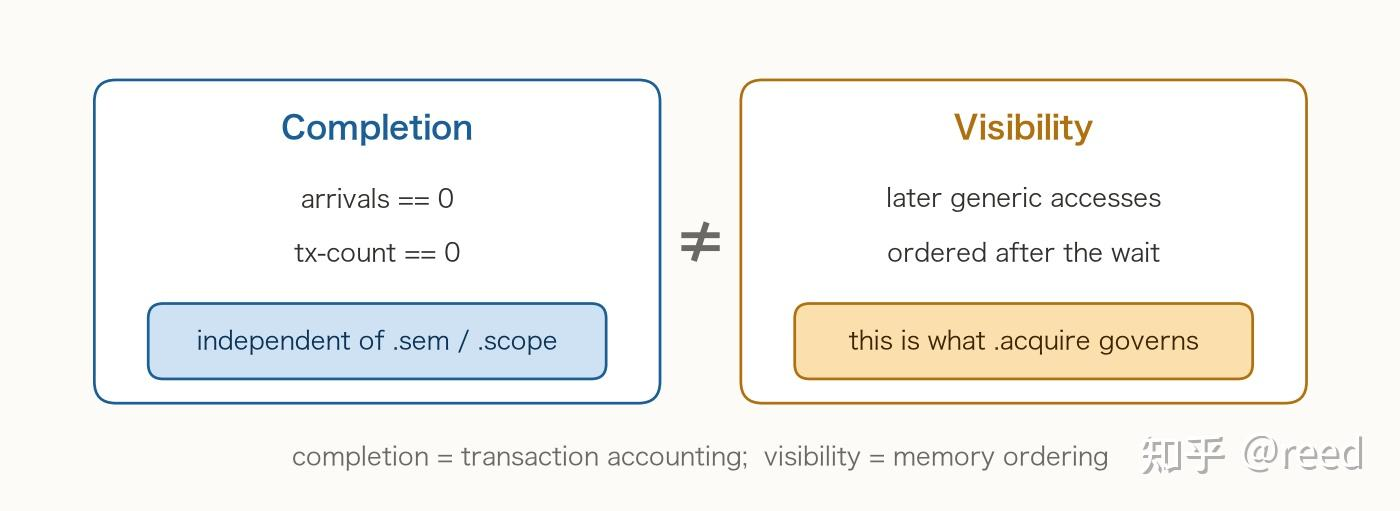
\includegraphics[width=0.9\textwidth]{figures/reed-mem-01-proxy/fig-06.jpg}
\caption{Figure 6. A barrier's two independent guarantees: completion by counting versus visibility by ordering.}
\end{figure}

完成状态由 mbarrier 计数决定。在本文使用的 \lstinline|layout::v0| 中，phase 翻转要求 pending arrivals 与 tx-count 两者都归零。所有被跟踪的异步操作字节都完成后，\lstinline|try_wait| 才返回 true；这一计数条件与 wait 上的 \lstinline|.sem| / \lstinline|.scope| 无关。

内存可见性由同步语义决定。\lstinline|.acquire| 约束 wait 返回后本线程的后续 generic 访问。

因此，仅跟踪异步字节是否完成时不需要额外内存语义；后续 generic 读取还需要被约束在 wait 成功之后时，才需要 acquire。两类保证分开后，modifier 可以按数据边逐项确定。这也是后文 Q1（完成）与 Q2（可见性）相互独立的原因。

\section{TMA 完成语义}

PTX 规定，\lstinline|cp{.reduce}.async.bulk| 完成后伴随一条隐式的 generic-async proxy fence：一旦完成被观测，其 async 写入结果即对 generic proxy 可见，因此该 async$\rightarrow$generic 数据边无需再执行双向 \lstinline|fence.proxy.async|。后续 generic 读仍需由 wait 上的 \lstinline|.acquire| 或独立的 \lstinline|fence.acquire| 约束在完成之后（PTX ISA，cp.async.bulk 与 Memory Consistency Model）。

这条 fence 是规范挂在 completion 机制上的，而不是由 release/acquire 推导出来的，因此它并不与 morally strong 的同 proxy 要求冲突：跨 proxy 的 causality 依然需要有东西来建立，只不过这一次由指令规范预先给定。哪些异步操作的完成带这条隐式 fence，要按各自的规范条目确认；不能因为存在这类例外，就指望 release/acquire 去覆盖其它跨 proxy 数据边。

这条隐式保证只有 async$\rightarrow$generic 方向。若同一缓冲区随后由新的 TMA 覆写，本轮 generic 读$\rightarrow$下一轮 async 写仍需单独建立 generic$\rightarrow$async ordering。其它异步写也必须按各自规范判断，不能直接套用 TMA 完成时的隐式保证。

PTX 给出的 canonical acquire pattern 把 fence 放在成功分支，避免在重试路径上重复执行：

\begin{lstlisting}
cp.async.bulk.mbarrier::complete_tx::bytes.relaxed.sys.b128 [dst], [M], size, [barrier];
mbarrier.try_wait.relaxed p, [barrier];
@p fence.acquire;
\end{lstlisting}

官方示例里对本地 SMEM 的 acquire 也采用同一写法：relaxed wait 加一条独立的 acquire fence。

\begin{lstlisting}
mbarrier.try_wait.relaxed.cluster.shared::cta.b64 complete, [addr], phase;
fence.acquire.sync_restrict::shared::cluster.cluster;
\end{lstlisting}

\section{典型数据边}

以下选取四种典型场景：同 proxy 消费、generic 读取、跨 CTA 的 mbarrier 交接和异步响应缓冲区的跨 proxy 复用。每条数据边都按同一套四步判定：完成（Q1）、消费方的 proxy 与可见性（Q2，含 tcgen05 等指令族的 execution ordering）、普通内存同步的 scope（Q3）与反向复用（Q4）；这些关系不能互相替代，四步的完整口径见后文“同步判定”。

\section{TMA 写入与 tcgen05.mma 消费}

TMA 写入与后续 async-proxy 消费位于同一 proxy，因此这条数据边不需要 proxy fence；mbarrier 的 tx-count 负责完成跟踪（Q1）。wait 上的 acquire 约束的是 wait 之后的 generic 访问，而 \lstinline|tcgen05.mma| 属 async proxy，其 ordering 不来自 acquire（Q2）。wait 成功后要发起异步 tcgen05 操作时，PTX canonical sequence 用 \lstinline|tcgen05.fence::after_thread_sync| 将其排在此前的 mbarrier execution-ordering operation 之后（PTX ISA，tcgen05 Memory Consistency Model: Canonical Synchronization Patterns）。

这里出现的是两种不同的定序：memory ordering 决定一次写在什么时候对读方可见，execution ordering 决定两条指令在各自的发射通路上谁先谁后。对这条数据边，TMA completion、tx-count 与同 proxy 规则共同保证 async 写入已经完成，relaxed wait 只负责观测完成状态；若后续改由 generic proxy 读取，还需要 acquire 约束后续访问。tcgen05 另需 execution ordering，因此这条专用 fence 不能被同一个 mbarrier wait 取代。mbarrier 的 phase 翻转是 SMEM 中的一次计数事件，\lstinline|try_wait| 返回只保证“计数已达成”；而 tcgen05 的操作数与执行走的是 Tensor Core 独立的发射通路，它并不自动排在这次计数事件之后。\lstinline|tcgen05.fence::after_thread_sync| 正是把随后的 tcgen05 操作显式排到先前那次 execution-ordering operation 之后，补上这条 wait 覆盖不到的顺序。这一位置是按指令族填的：mbarrier 负责完成跟踪，并可通过 acquire 传递普通内存效应；凡是自带独立发射通路的异步指令族，还要在这里补上属于自己的 execution ordering，具体指令由各自的规范给出。

以 Blackwell 2SM（\lstinline|cta_group::2|）主循环为例，两个 CTA 各发一条 TMA 搬运各自的半份 tile 到本地 SMEM，MMA 由 CTA pair 共同执行。以下 PTX 仅用于表达 issuer、完成信号与 execution ordering 的关系：省略 \lstinline|tcgen05.mma| 的部分强制操作数，示例假设每个 CTA 只有一个参与线程，不作为可直接汇编的完整程序。CTA 内有多个线程时，\lstinline|barrier.cluster.arrive| 必须由所有未退出线程各执行一次，否则 barrier 无法完成。

\begin{lstlisting}
// p_cta_leader：每个 CTA 恰好一个 elected thread
// p_pair_issuer：CTA pair 中恰好一个 tcgen05 issuer；本例选择 CTA0 的 elected thread
// %r_mbar：本 CTA 的 mbarrier 的 shared 地址

// CTA0 elected thread 登记两条 TMA 的总事务字节数
@p_pair_issuer mbarrier.arrive.expect_tx.relaxed.cta.shared::cta.b64
               _, [%r_mbar], tx_bytes_total;
barrier.cluster.arrive.relaxed;
barrier.cluster.wait;

// 清除 peer bit：cta_group::2 的完成信号按 CTA-Pair 归并，统一记到 CTA0
and.b32 %r_mbar_pair, %r_mbar, 0xFEFFFFFF;

// 每个 CTA 仅由 elected thread 发起一条 TMA 写入本地 SMEM
@p_cta_leader cp.async.bulk.tensor.2d.shared::cta.global
 .mbarrier::complete_tx::bytes.cta_group::2.L2::cache_hint
 [smem], [tmap, {c0,c1}], [%r_mbar_pair], hint;

// CTA0 的 pair issuer 等待并发起一次 tcgen05.mma
@!p_pair_issuer bra mmaDone;
waitLoop:
mbarrier.try_wait.parity.relaxed.cluster.shared::cta.b64 P, [%r_mbar], phase;
@!P bra waitLoop;
tcgen05.fence::after_thread_sync;
tcgen05.mma.cta_group::2.kind::f16 [taddr], adesc, bdesc, idesc, enable-input-d;
mmaDone:
\end{lstlisting}

\section{完成信号与发起粒度}

多 CTA 协同还包含两个与 sem / scope 无关的约束：完成信号的目标 CTA 与 MMA 的发起粒度。

完成信号路由由 mbarrier 地址决定，只有持有该 mbarrier 的 CTA 能够执行 wait。在 Blackwell 上，\lstinline|cta_group::2| 的完成信号落到 CTA-Pair 中的哪个 CTA，取决于 mbar 所在 SMEM 属于该 pair 的偶数号还是奇数号 CTA——mbarrier 既可以与目标 SMEM 同属一个 CTA，也可以位于其 peer-CTA。因此 CUTLASS 主动把 peer bit 清 0，让两个 CTA 的完成信号统一记到 CTA0。

\begin{figure}[htbp]\centering
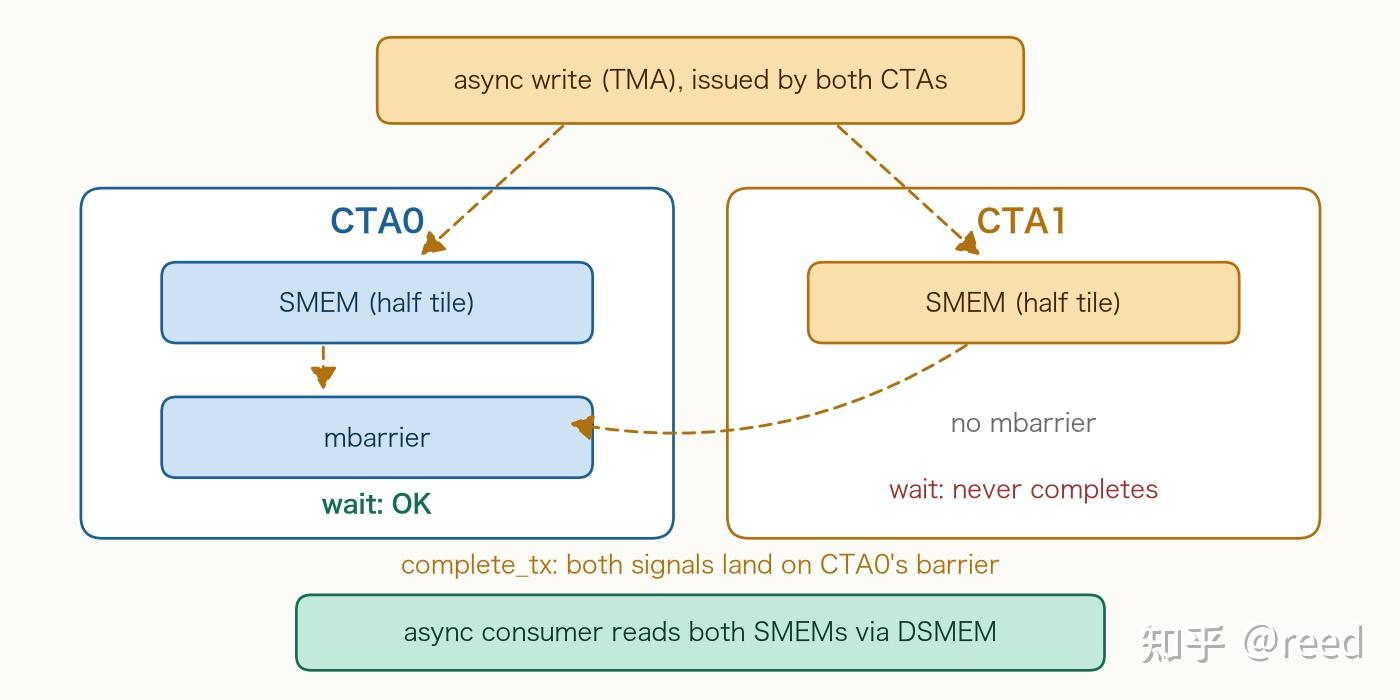
\includegraphics[width=0.9\textwidth]{figures/reed-mem-01-proxy/fig-07.jpg}
\caption{Figure 7. Routing of an async write's completion signal: only the CTA holding the barrier may wait.}
\end{figure}

图中两个 CTA 各把自己那半份 tile 写入本地 SMEM，但完成信号都被引导到 CTA0 的 mbarrier；CTA1 没有屏障，只有持有屏障的 CTA0 能够 wait，随后异步消费者经 DSMEM 读取两份 SMEM。

指令发起粒度要求 \lstinline|cta_group::2| 操作由 CTA pair 中的单个线程发起，且 peer CTA 必须处于 active、未退出状态。若一个 warp 的 32 个线程都执行该指令，就不满足“单线程发起”的规范要求，其行为不被 PTX 定义，不应依赖任何具体表现。

\section{TMA 写入与 generic 读取}

数据由线程使用 generic load（\lstinline|ld.shared| / \lstinline|ldmatrix| / \lstinline|ld.global|）消费时，wait 成功后需要 acquire（Q2 落在 generic load 分支）。scope（Q3）取决于建立 release/acquire 关系的两个端点是否跨 CTA；数据地址位于本地还是远端是判断端点位置的一项依据，但不是唯一条件。

\begin{lstlisting}
waitLoop:
mbarrier.try_wait.parity.shared::cta.b64 P, [mbar], phase; // 默认 = .acquire.cta
@!P bra waitLoop;
ld.shared.v4.b32 {r0,r1,r2,r3}, [smem]; // 或 ldmatrix.sync.aligned.m8n8.x4.shared.b16
\end{lstlisting}

可以采用以下两种写法：

\begin{lstlisting}
// (i) 单条指令即可（默认 .acquire.cta）
mbarrier.try_wait.parity.shared::cta.b64 P, [mbar], phase;

// (ii) relaxed wait + success-path acquire fence
mbarrier.try_wait.parity.relaxed.cluster.shared::cta.b64 P, [mbar], phase;
@!P bra waitLoop;
fence.acquire.sync_restrict::shared::cluster.cluster;
\end{lstlisting}

TMA 向本 CTA 的 SMEM 写入、且消费者也在本 CTA 时，\lstinline|.acquire.cta| 足以覆盖本地读取；若消费者依赖另一 CTA 的普通写入，或通过 DSMEM 读取对端数据，则 release 与 acquire 都必须使用 \lstinline|.cluster|。TMA 的 complete-tx 已带 \lstinline|.release.cluster|（这是 \lstinline|cp.async.bulk.tensor| 规范固定的语义，不由前述 arrive/wait 默认值决定），普通线程的 mbarrier arrive 则需要显式选择与 consumer 匹配的 scope。

作为反向数据边（Q4）的对照，generic 写入随后由异步操作读取时，程序序仍不能替代 proxy ordering。TMA 完成已经提供 async$\rightarrow$generic 的隐式 proxy ordering，因此该方向不需要额外的 \lstinline|fence.proxy.async|；反向的 generic$\rightarrow$async 数据边仍需显式建立：线程先用 \lstinline|st.shared| 把数据写进 SMEM，再让异步操作经 async proxy 读这块 SMEM 时（例如把它作为 TMA store 的源，或作为 tcgen05 读 SMEM 的输入），需要执行 \lstinline|fence.proxy.async.shared::cta|，即 CUTLASS 的 \lstinline|fence_view_async_shared()|。

写入与异步读取由同一线程按程序序发起，但二者分别位于 generic 与 async proxy，morally strong 仍不成立。该场景不涉及跨线程同步，只需要建立 generic$\rightarrow$async 的 proxy ordering，直接说明了 proxy 与线程维度相互独立。

需要区分的一点是：TMA 使用的 tensormap 描述符本身不属于这条 SMEM 数据边，它需经 \lstinline|fence.proxy.tensormap::generic| 一类机制发布，不能与上面这条 \lstinline|fence.proxy.async.shared::cta| 混为一谈。

\section{跨 CTA 的 mbarrier 交接}

mbarrier 对象可以位于远端 CTA 的 SMEM（\lstinline|.shared::cluster|），但 wait 只能作用于本地 mbarrier 对象——PTX 的远端地址支持矩阵中，\lstinline|.shared::cluster| 只支持 \lstinline|arrive / arrive_drop / expect_tx / complete_tx|，其余（含 init / \lstinline|test_wait| / \lstinline|try_wait|）一律 Not supported，对远端对象执行 wait 不被 PTX 支持、行为未定义（PTX ISA，§9.7.14.16.11 mbarrier Instructions）。scope 是否升级，取决于是否通过 mbarrier 在跨 CTA 的执行端点之间交接普通内存效应；只传递计数、phase 或资源状态时不需要 cluster 级 release/acquire。

在 2SM empty barrier 中，MMA 消费完成后 producer 复用 SMEM buffer，odd CTA 远程 arrive 到 even CTA 的 barrier（CUTLASS \lstinline|umma_arrive_2x1SM_sm0|，barrier.h:912）：

\begin{lstlisting}
// (i) MMA 的完成跟踪：由 commit 直接登记到 empty barrier，同时带生产侧 ordering
// .cta_group 必选，且须与同一 kernel 内 tcgen05.mma 的 cta_group 一致
tcgen05.commit.cta_group::2.mbarrier::arrive::one.shared::cluster.b64 [%r_mbar_pair];

// (ii) odd CTA 远程 arrive 到 even CTA 的 barrier（CUTLASS 中即 umma_arrive_2x1SM_sm0）
mbarrier.arrive.shared::cluster.b64 _, [%r_mbar_pair];  // %r_mbar_pair 同前，已清除 peer bit
                                                        // 未写 sem / scope，默认 = .release.cta
\end{lstlisting}

两种写法的职责不同。\lstinline|tcgen05.commit.mbarrier::arrive::one| 让 mbarrier 跟踪此前异步 \lstinline|tcgen05.mma| 的完成，并同时提供生产侧所需的 execution ordering；第（ii）种只贡献一次 arrive，必须由已经确认完成的线程发出。若异步操作是 \lstinline|tcgen05.ld| 这类需要先 wait 再交给对端的场景，PTX canonical 给出的是 \lstinline|tcgen05.wait| 加 \lstinline|tcgen05.fence::before_thread_sync|，再接 \lstinline|mbarrier.arrive|：这条 fence 只补 execution ordering，不承担完成跟踪，不能与 commit 互换。mbarrier 在这里仅传递“SMEM buffer 可以复用”这一资源状态，不交接普通内存数据，因此不需要 cluster 级 release/acquire；现有默认语义可以工作，显式 relaxed 也足以表达这条计数关系。

这条边同时给出了反向复用（Q4）的另一种情形：\lstinline|tcgen05.mma| 对 SMEM 的读取与下一轮 TMA 的写入都发生在 async proxy 内部，反方向的复用因此不跨 proxy，不需要 proxy fence，但仍须由上述 specialized execution ordering 把消费完成排到复用信号之前。只有当本轮消费改为线程的 generic 读取时，反向边才跨 proxy，也才需要下一节讨论的 release proxy fence。

当生产者需要把本 CTA 的普通内存写交给对端 CTA 的 waiter 时，构成 DSMEM 数据交接，release 与 acquire 必须两侧同时使用 \lstinline|.cluster|：

\begin{lstlisting}
mbarrier.arrive.release.cluster.shared::cluster.b64 _, [remAddr]; // 生产者
mbarrier.try_wait.parity.acquire.cluster.shared::cta.b64 P, [bar], phase; // 消费者
\end{lstlisting}

单边升级无效。CuTe DSL 对这一取舍有一段直接的注释（mbar.py:437-442），大意是：远程 arrive 在形式上应当使用 cluster scope 以获得跨 CTA 的内存模型排序；保留 CTA 默认值是因为现有协议只依赖屏障计数，且 cluster scope 在那里实测更慢；做 DSMEM 数据交接时应显式传 CLUSTER。

\section{异步响应缓冲区复用}

缓冲区在本轮由 generic proxy 读取、下一轮由 async proxy 覆写时（Q4），需要 generic$\rightarrow$async 的 release proxy fence，把本轮读取排在下一轮异步写之前。这条 fence 不能移到 wait 上，因为 wait 的 acquire 只约束其后的访问。TMA 完成时附带的隐式 fence 只覆盖 async$\rightarrow$generic 的相反方向，因此缓冲区复用时同样需要这一 release fence。

Cluster Launch Control（CLC，运行时把待处理的 CTA 动态分派给 cluster 的机制）流水线中的 \lstinline|clc_info[stage]| 是一块复用的 16 字节响应缓冲区：\lstinline|try_cancel| 异步写入响应，线程等待 mbarrier 后用 \lstinline|ld.shared.b128| 读取 handle，再由 release proxy fence 把本轮读取排在下一轮 \lstinline|try_cancel| 之前。

该 fence 必须保留在 generic 读与下一轮 async 写之间。 该缓冲区被两个 proxy 交替访问：\lstinline|try_cancel| 在 \lstinline|.multicast::cluster::all| 下以 weak async-proxy writes（未定序的 async proxy 写）把响应写到 cluster 内每个 CTA 各自的本地 SMEM（PTX ISA，\lstinline|clusterlaunchcontrol.try_cancel|），\lstinline|ld.shared| 读则属 generic proxy，跨 proxy 时 morally strong 不成立。如果缺少 generic$\rightarrow$async 的 release proxy fence，下一轮新的 async 写可能覆盖上一次 \lstinline|ld.shared| 仍在读取的值，读到撕裂的 handle、解出错误的 ctaid，最终可能表现为错误的 tile 分配。

该 fence 约束的是“本次 generic 读$\rightarrow$下次迭代 async 写”。wait 上的 \lstinline|.acquire| 只约束 wait 之后的访问；这里需要 release 语义，将 fence 之前的 generic 读排在 fence 之后的 async 写之前。

\begin{figure}[htbp]\centering
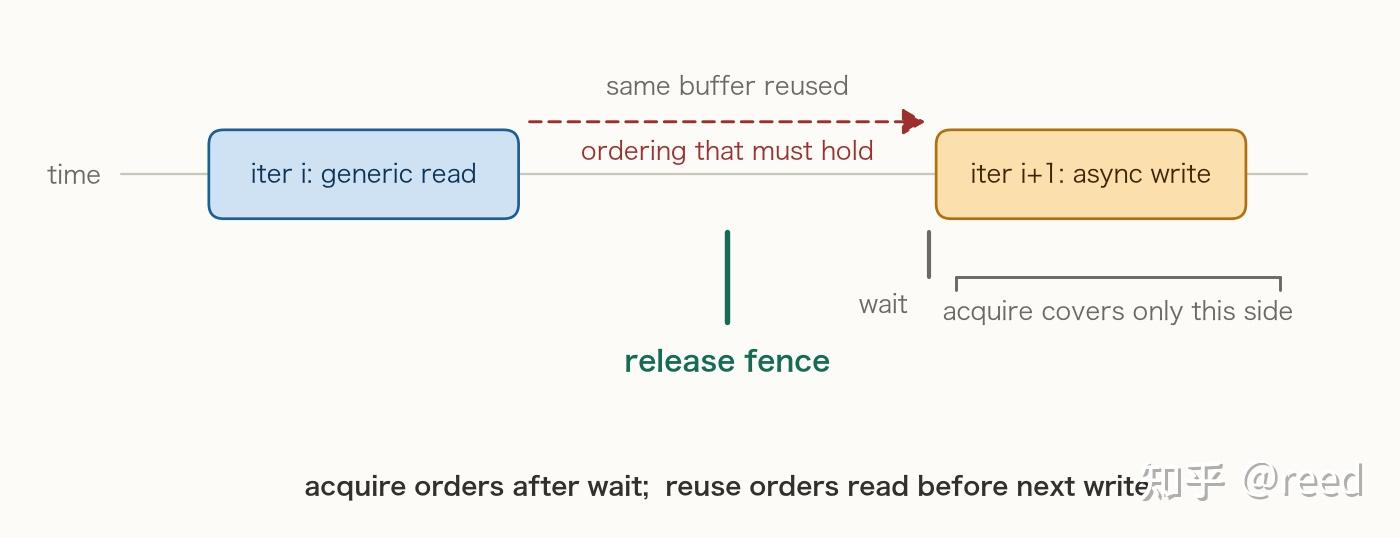
\includegraphics[width=0.9\textwidth]{figures/reed-mem-01-proxy/fig-08.jpg}
\caption{Figure 8. A reused async response buffer: why the release fence cannot be moved onto the wait.}
\end{figure}

图中红色虚线是必须保持的“本轮读$\rightarrow$下轮写”顺序，绿色竖线（release fence）压在两者之间；右侧的 wait 及其 acquire 只笼罩它之后的一段，无法覆盖到下一轮的写，这正是 fence 不能挪到 wait 上的原因。

\section{CLC 官方示例中的同步关系}

官方示例的关键几行：

\begin{lstlisting}
waitLoop:
 mbarrier.try_wait.parity.acquire.cluster.shared::cta.b64 complete, [mbar], phase;
 @!complete bra waitLoop;
 ld.shared.b128 handle, [addr];
 // ↓ 保护“本次 generic 读”先于“下次 async 写”
 fence.proxy.async::generic.release.sync_restrict::shared::cta.cluster;
 barrier.cluster.arrive.relaxed;
 barrier.cluster.wait;
 // 与上一轮各 CTA 的 release proxy fence 配对；方向仍为 generic→async
 fence.proxy.async::generic.acquire.sync_restrict::shared::cluster.cluster;
\end{lstlisting}

该示例包含三个独立约束。第一，\lstinline|mbarrier.try_wait.acquire.cluster| 既等待 CLC 响应完成，也阻止随后的 generic \lstinline|ld.shared| 越过 wait。第二，本轮读完 handle 后，release proxy fence 建立 generic$\rightarrow$async ordering；cluster 会合后的 acquire proxy fence 与各 CTA 的 release sequence 配对，把上一轮各 CTA 的 generic 读排在当前迭代的 async 写之前。两条单向 fence 的 proxy 方向相同，区别在跨线程同步中的 release/acquire 角色。第三，multicast 下 \lstinline|try_cancel| 由 elected CTA 发起，却写入每个 CTA 各自的本地 SMEM，因此这对单向 fence 使用 \lstinline|.cluster| scope。

\section{同步判定}

同步选择分成两层。第一层确定需要建立的关系：本线程访存顺序使用 fence，线程集合会合使用 barrier，事件、资源状态或异步事务完成使用 mbarrier；若同一条数据边跨 proxy，还要按实际方向增加 proxy ordering。图 5 给出三类原语的职责边界，图 9 则把一条异步数据边的判定拆成依次确认的四步。

\begin{figure}[htbp]\centering
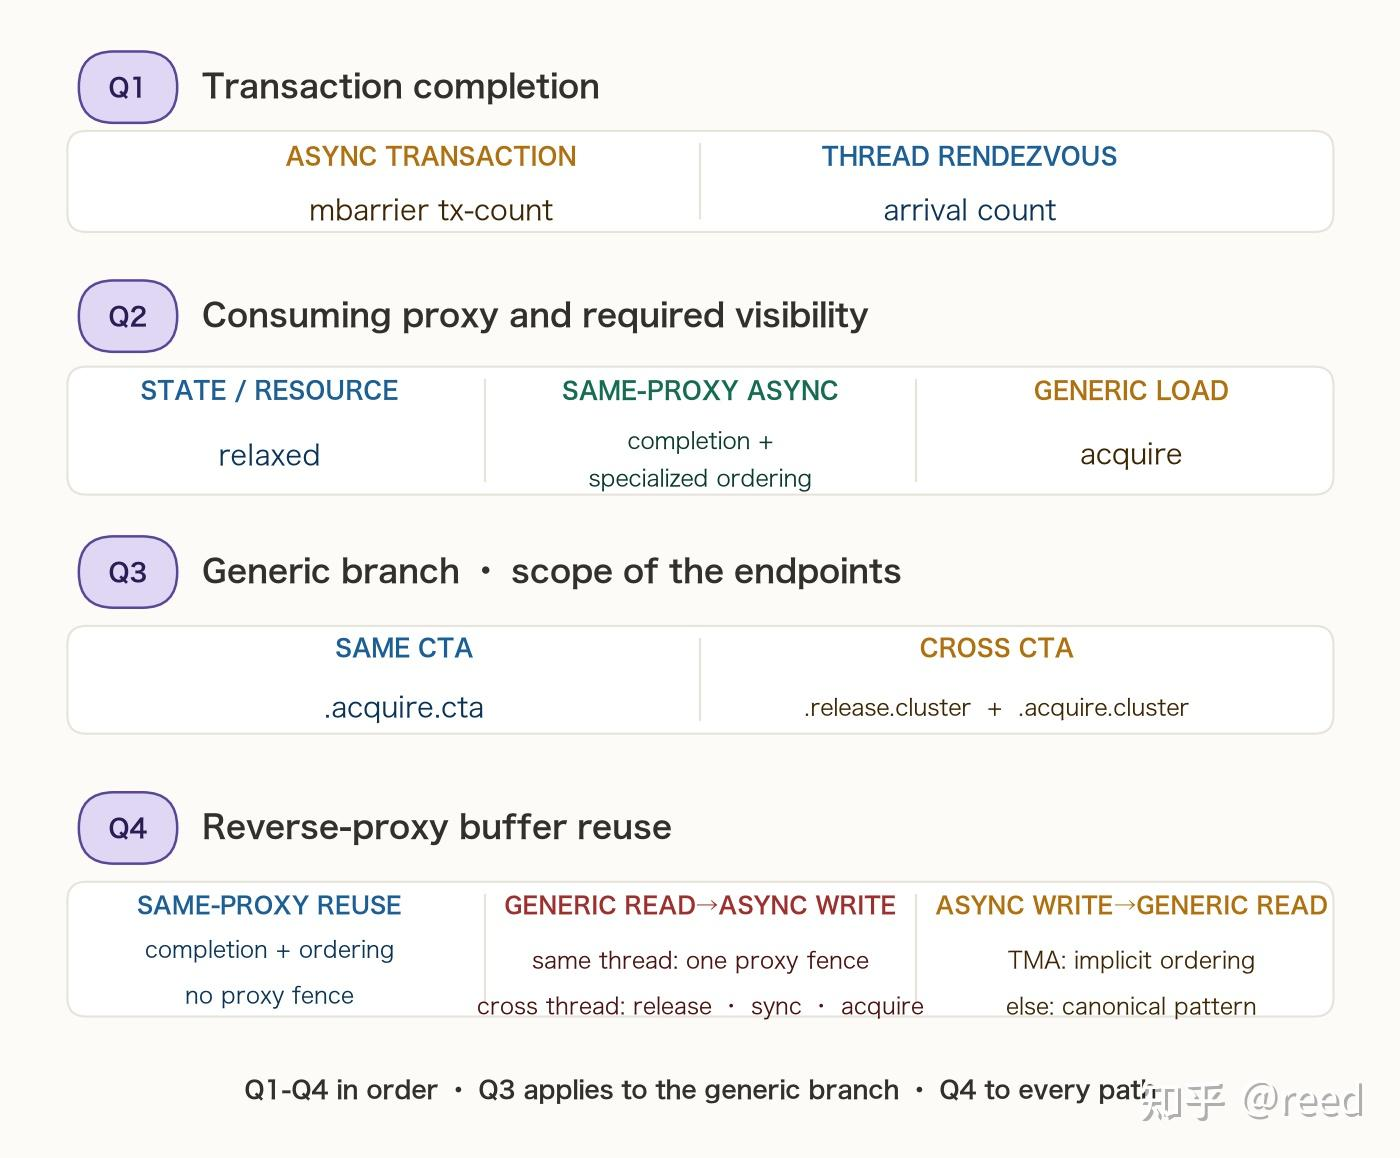
\includegraphics[width=0.9\textwidth]{figures/reed-mem-01-proxy/fig-09.jpg}
\caption{Figure 9. Four checks for ordering an async data edge.}
\end{figure}

Q1 完成：异步事务或事件的完成由计数机制判定——TMA 用 tx-count，线程会合用 arrival count，\lstinline|try_wait| 返回 true 即代表当前 phase 的计数条件已满足；这一步与 sem / scope 无关。

Q2 消费方的 proxy 与可见性：这一步确定 wait 成功后由谁、经哪个 proxy 消费，以及消费方必须看到的内容。只传递 phase 或资源状态时 relaxed 足够；同 proxy 的异步消费者（如 \lstinline|tcgen05.mma|）依赖完成计数，并按指令族补 specialized execution ordering 及其 scope（如 canonical 里的 relaxed wait 加 \lstinline|.cluster|，再接 \lstinline|tcgen05.fence::after_thread_sync|）；generic load 则需要 acquire。

Q3 普通内存同步的 scope：仅当数据边需要通过 release/acquire 传递普通内存效应时单独判断，由两个同步端点是否跨 CTA 决定 \lstinline|.cta| 还是两侧 \lstinline|.cluster|。异步指令族自身的 execution-ordering scope 已在 Q2 中处理。

Q4 反向复用：独立作用于所有分支，先看本轮消费所经的 proxy。若消费也走 async proxy（如 \lstinline|tcgen05.mma| 直接读 SMEM），反向边是 async$\rightarrow$async，同 proxy，不需要 proxy fence；但仍须由 \lstinline|tcgen05.commit|（或 \lstinline|tcgen05.fence::before_thread_sync| 加显式完成等待）把消费的完成与 execution ordering 一起排到复用信号之前。若本轮是 generic 读、下一轮由 async proxy 覆写，反向边才跨 proxy：同一线程使用一条 generic$\rightarrow$async proxy fence；不同线程则由 reader 侧 release proxy fence、线程间同步和 writer 侧 acquire proxy fence 组成，两条单向 fence 的 proxy 方向都为 generic$\rightarrow$async。至于 async 写$\rightarrow$generic 读方向，\lstinline|cp.async.bulk*| 的完成已提供隐式保证，其它异步操作按各自的 canonical completion pattern 处理。

四步之外，还有两点贯穿始终：mbarrier 对象可以位于远端 CTA 的 SMEM，但 \lstinline|test_wait| / \lstinline|try_wait| 只能访问本 CTA 的 mbarrier；地址空间、同步 scope 与 proxy 方向三者互不蕴含，需要分别确认。

\section{常见错误}

Q1 的错误集中在完成机制与对象归属。 非持有 CTA 对远端 mbarrier 执行 wait 不受 PTX 支持；\lstinline|bar.sync| 与 \lstinline|barrier.cluster.wait| 不跟踪 TMA 事务；\lstinline|barrier.cluster| 只要还有未退出线程没有 arrive 就无法完成；\lstinline|cta_group::2| 操作也不能由多个线程重复发起。

Q2 / Q3 的错误集中在 scope 与地址空间。 跨 CTA 传递普通内存效应时，生产侧缺少 release、只升级 wait 不能建立同步；\lstinline|.shared::cluster| 是地址空间，不等于 \lstinline|.scope::cluster|；省略 \lstinline|fence.mbarrier_init.release.cluster| 会让远端 CTA 观察到未发布的 barrier 状态。语法上，\lstinline|.sem| 与 \lstinline|.scope| 必须成对出现，\lstinline|.acquire| 也不能和 \lstinline|sync_restrict::shared::cta| 组合。

Q2 / Q4 的错误集中在 proxy、execution ordering 与缓冲区复用。 \lstinline|fence.proxy.to::from| 的方向始终由 from $\rightarrow$ to 决定，不随 release/acquire 反转；acquire 不能替代 proxy fence；wait 后直接发起 tcgen05、省略 \lstinline|after_thread_sync| 会缺少 specialized execution ordering；generic 读取后的缓冲区若由 async proxy 复用，也不能省略反向 proxy fence。不同虚拟地址访问同一位置仍可能形成 \lstinline|.alias| proxy，不能按普通 generic 同址访问处理。

\section{总结}

内存模型规定可见性与顺序，具体保证由编译器、执行流水线和缓存一致性机制共同实现。PTX 在此基础上进一步暴露线程集合与访问方法两个维度：scope 描述同步覆盖的线程，proxy 描述内存访问方法。morally strong 的三条件说明这两个维度正交——跨 proxy 数据边需要单独建立 causality order，即便操作出自同一线程也不例外；若操作还分属不同线程，则同时满足 release/acquire 与 scope 条件。

mbarrier 的 phase 由 arrival count 与 tx-count 推进，完成状态与内存可见性相互独立。只传递资源状态时可以使用 relaxed；交接普通内存数据时，需要按执行端点选择 sem 与 scope。TMA 完成附带的隐式 fence 只覆盖 async$\rightarrow$generic 方向，generic 读到下一轮 async 覆写仍需 generic$\rightarrow$async ordering。

fence 约束访存顺序；CUDA barrier 同时完成 collective rendezvous 与参与线程间的普通内存定序，但不跟踪 TMA 等异步事务；mbarrier 将 arrival 和 wait 拆开，可用于线程子集的 split-phase 会合，也可跟踪资源状态或异步事务完成，并按 sem / scope 选择是否传递普通内存效应。

落到具体一条数据边，判定就是图 9 的四步：Q1 确认事务完成，Q2 确定消费方的 proxy 与可见性，并按异步指令族补 execution ordering，Q3 按普通内存同步端点的线程范围选择 scope，Q4 判断缓冲区的反向复用是否跨 proxy；同 proxy 时保留指令族所需的完成与 execution ordering，跨 proxy 时再补反向 proxy fence。

\section{参考}

Hans-J. Boehm, Sarita V. Adve, Foundations of the C++ Concurrency Memory Model, PLDI 2008 \url{https://www.cs.toronto.edu/~pekhimenko/courses/csc2231-f17/Papers/C++Consistency.pdf}

Vijay Nagarajan et al., A Primer on Memory Consistency and Cache Coherence, 2nd Edition \url{https://directory.doabooks.org/handle/20.500.12854/97841}

NVIDIA, Parallel Thread Execution ISA 9.3: Memory Consistency Model; fence; bar; mbarrier; cp.async.bulk; tcgen05; \lstinline|clusterlaunchcontrol.try_cancel| \url{https://docs.nvidia.com/cuda/parallel-thread-execution/index.html}

NVIDIA, CUDA Programming Guide: Synchronization Functions; Asynchronous Barriers; Asynchronous Data Copies \url{https://docs.nvidia.com/cuda/cuda-c-programming-guide/}

NVIDIA CUTLASS, main: \lstinline|include/cute/arch/barrier.h|, \lstinline|include/cute/arch/copy_sm90_desc.hpp|, SM100 collective implementations \url{https://github.com/NVIDIA/cutlass}

LLVM, NVPTX Usage: mbarrier, proxy fence and tcgen05 intrinsics \url{https://llvm.org/docs/NVPTXUsage.html}

cute 之 Hopper MBarrier \url{https://zhuanlan.zhihu.com/p/1962636004235153810}
